\documentclass[11pt,letterpaper,twoside]{article}
\usepackage[english]{babel}
\usepackage{amssymb,amsmath}
\usepackage{fancyhdr}
\usepackage{graphicx}
\usepackage{wrapfig}

 \oddsidemargin  0in \evensidemargin 0in
 \topmargin   -0.25in \headheight 0.25in \headsep 0.25in
 \textwidth   6.5in \textheight 8.75in \marginparsep 0pt \marginparwidth 0pt
 \parskip 1ex  \parindent 0ex \footskip 20pt

\newfont{\bssten}{cmssbx10}
\newfont{\bssnine}{cmssbx10 scaled 900}

%%%%%%%%%%%%%%%%%%%%%%%
\newcommand{\whatizit}{Lecture 19: Inference for Means and the $t$-Distribution}
%%%%%%%%%%%%%%%%%%%%%%%


\pagestyle{fancy}  
\fancyhead{\bssnine STOR 155,  \whatizit}
\fancyhead[RE]{} \fancyhead[LO]{}
\fancyhead[LE]{\bssnine \thepage} \fancyhead[RO]{\bssnine \thepage}
\lfoot{} \cfoot{} \rfoot{}   


\newcommand{\var}{\mathrm{Var}}



\begin{document}



\thispagestyle{empty} \vspace*{-0.75in}

{\bssten STOR 155: Introduction to Data Models and Inference \hfill June 18, 2024 \\
Prof. Will Lassiter  \hfill Page 1 of \pageref{totalpag}}
\vspace{10pt}
\begin{center} {{\Large \bf \whatizit}} \end{center}

First example: Heights of U.S.\ women \vspace{60pt}

\begin{center}

\includegraphics[scale=0.8]{images/heights.png}
\end{center}

{\bf Sampling distribution of a sample mean}

\newpage

Example: The distribution of prices of snack-food items sold by a large supermarket chain is approximately normal with mean $\mu = \$3.34$ and standard deviation $\sigma = \$0.12$.

\begin{itemize}

\item What is the probability that a randomly chosen snack-food item costs less than \$3.25? \vspace{60pt}

\item Now take a SRS of 25 snack-food items and compute the mean cost.  What is the probability that $\bar{x}$ is less than \$3.25? \vspace{80pt}

\end{itemize}

Even if the parent population is not normally distributed, the sampling distribution of $\bar{x}$ is still approximately normal when ... \vspace{80pt}

\begin{center}
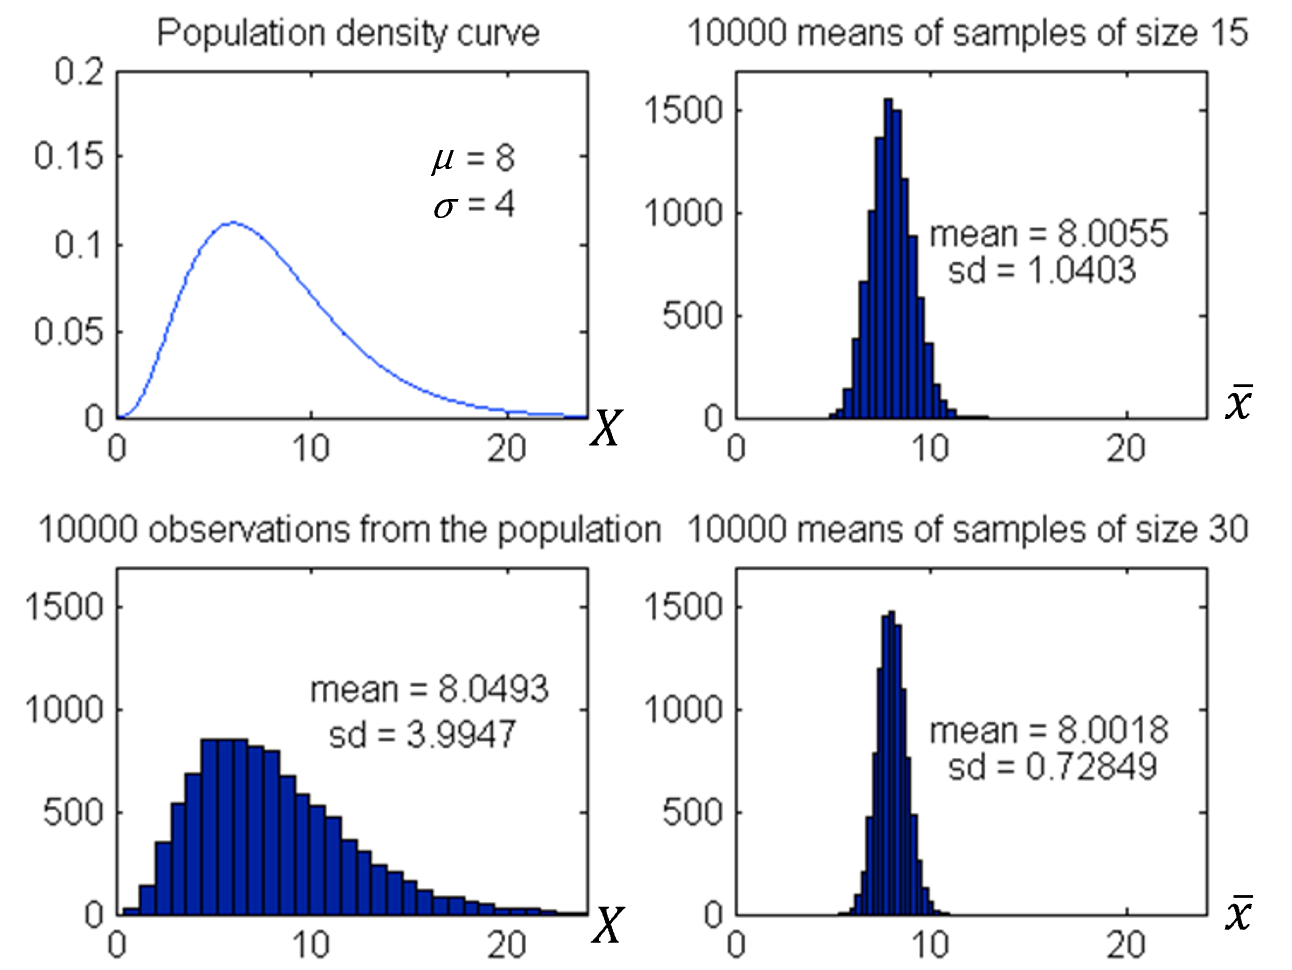
\includegraphics[scale=0.7]{images/skewed.png}
\end{center}

\newpage

If we know population standard deviation $\sigma$ (unlikely) and want to run an observed sample mean $\bar{x}$ through a hypothesis test, we would compute ... \vspace{60pt}

If we don't know $\sigma$ (likely), we must instead compute ... \vspace{80pt}

\begin{center}
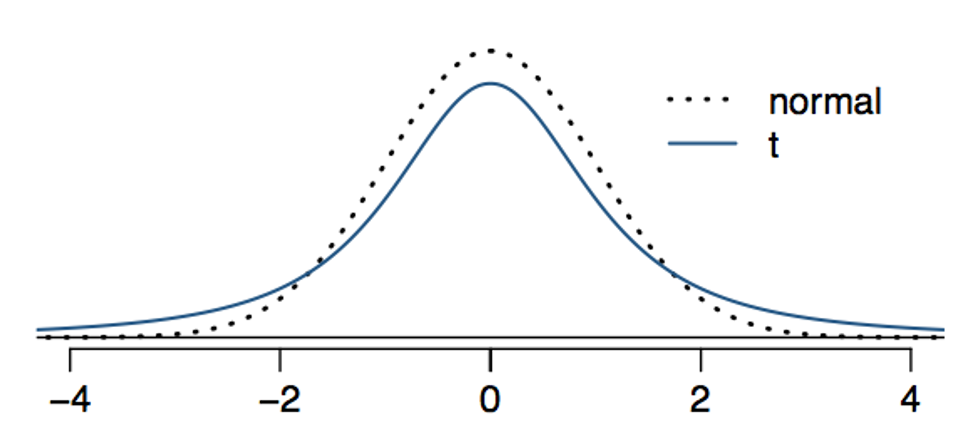
\includegraphics[scale=0.9]{images/t.png}
\end{center}

\begin{center}
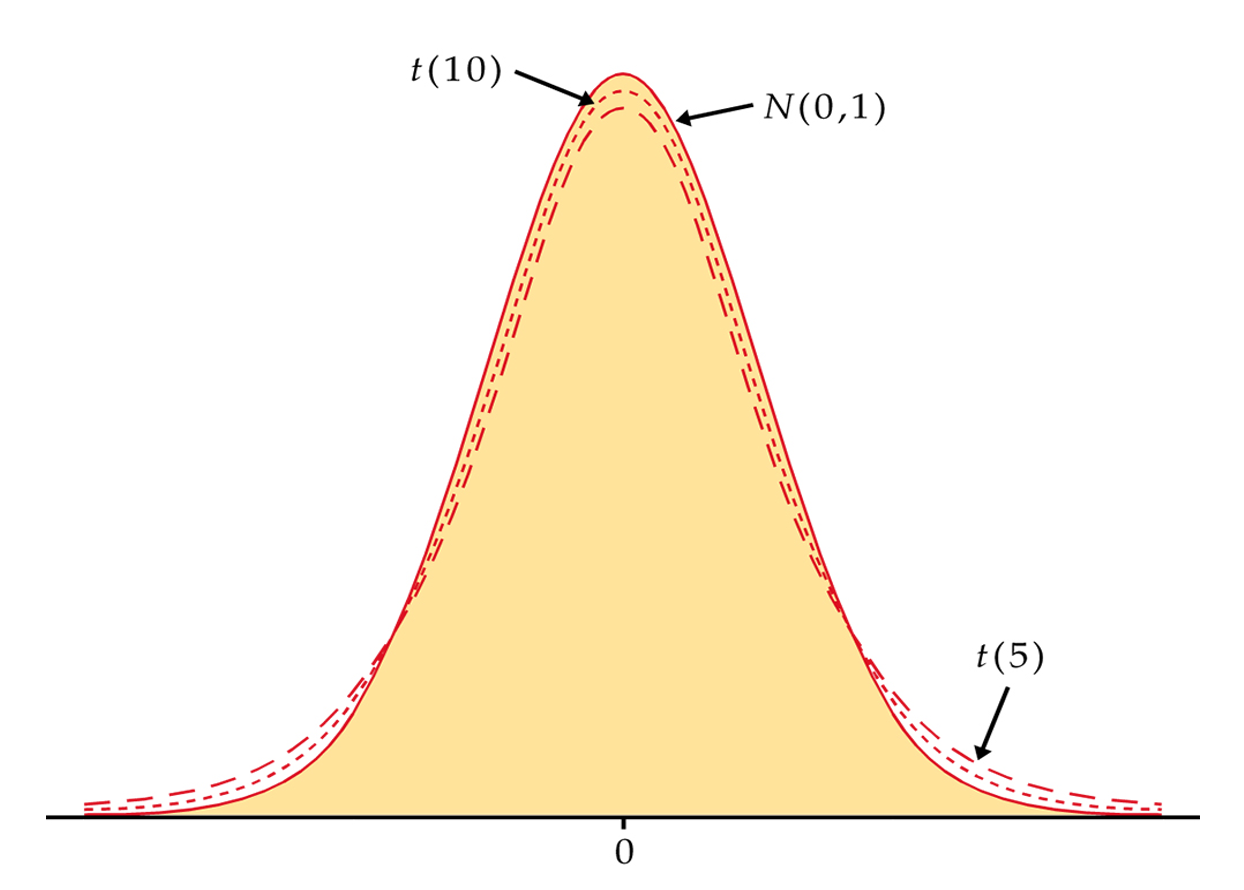
\includegraphics[scale=0.7]{images/t2.png}
\end{center}

\newpage

{\bf Confidence intervals using the $t$-distribution}

\begin{center}
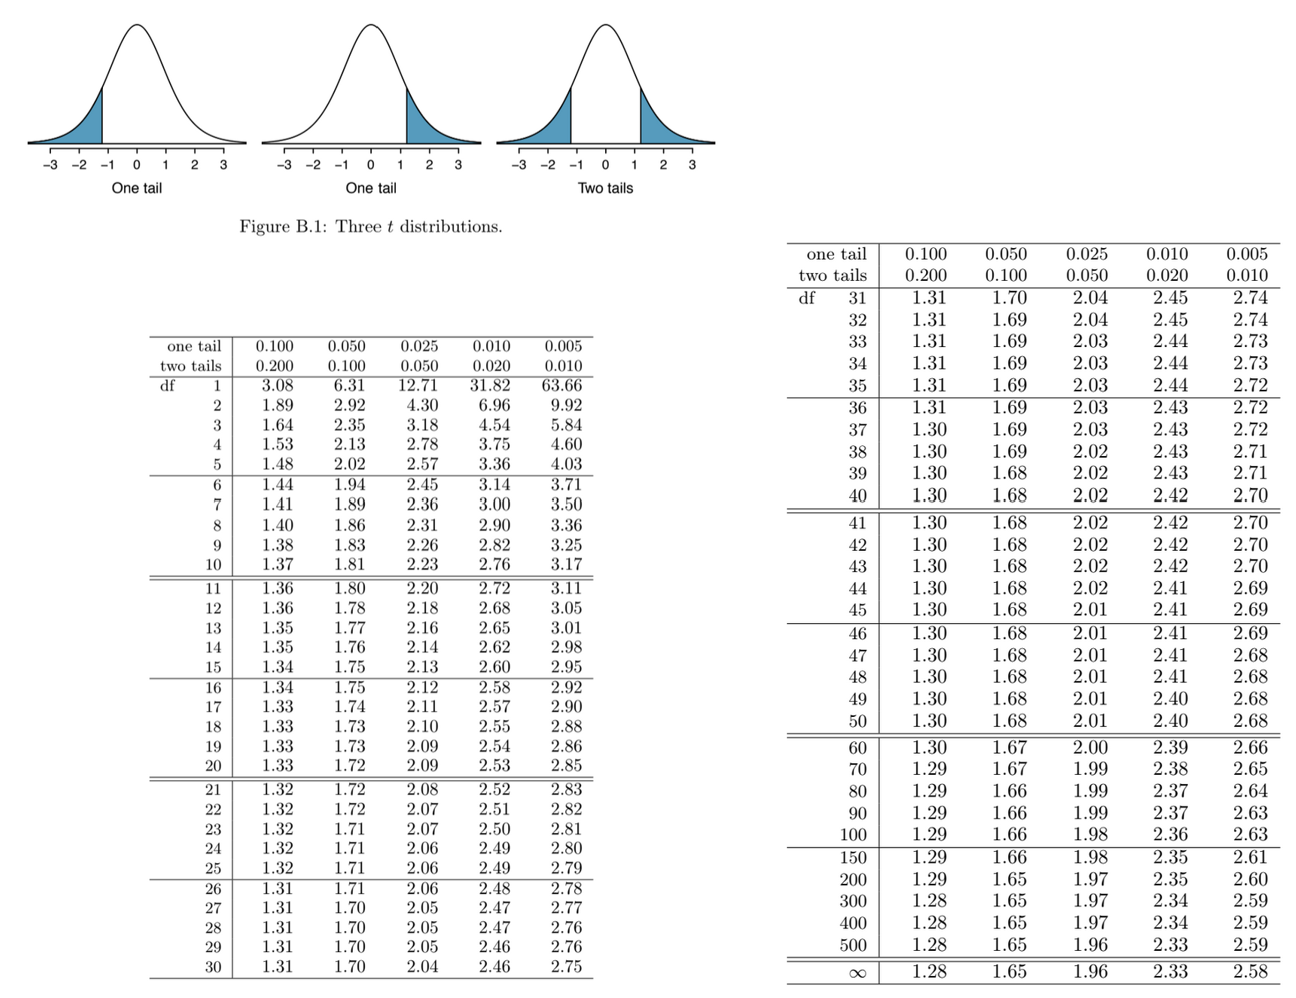
\includegraphics[scale=0.9]{images/table.png}
\end{center}

Example: An investor would like to estimate the average return on investment (ROI) for companies that won quality awards last year.  He takes a random sample of 40 award-winning companies and finds that $\bar{x}=14.75\%$ and $s=8.18\%$. Construct a 95\% CI for $\mu$, the average return on investment for all quality award-winning companies.

\newpage

Origins of the $t$-distribution: William Sealy Gossett

\begin{center}
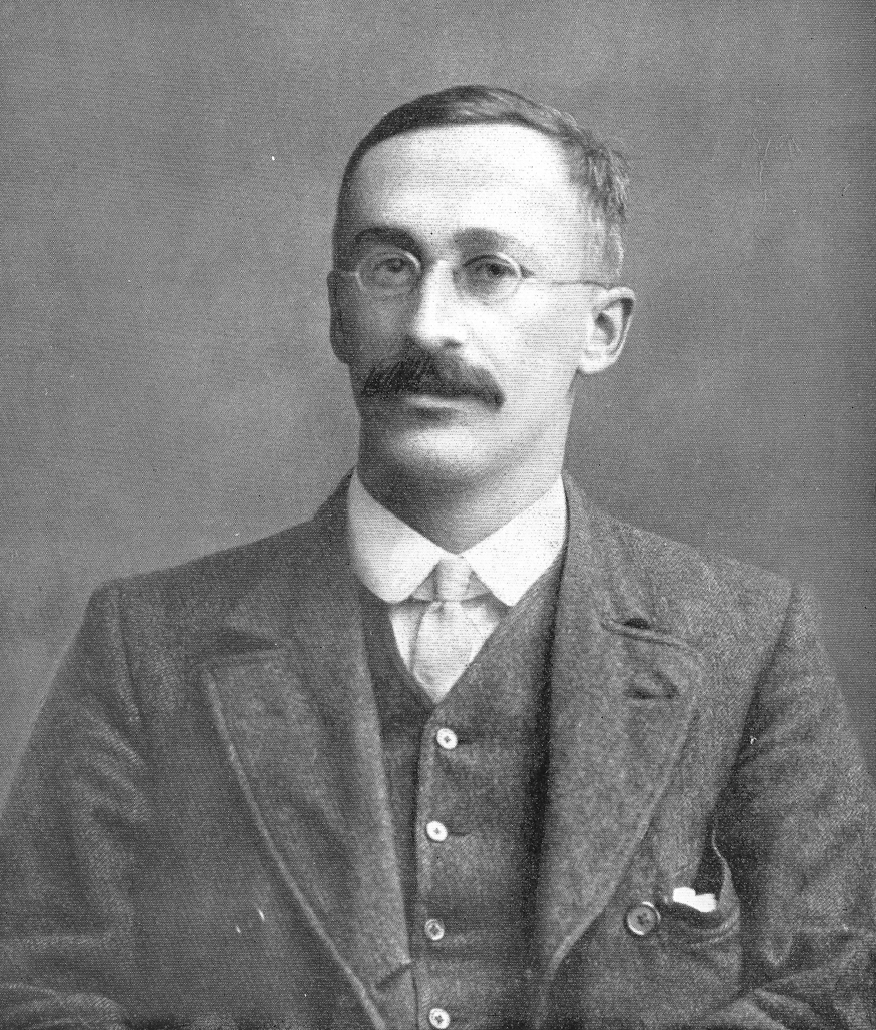
\includegraphics[scale=0.4]{images/gossett.png}
\end{center}

Example: It has been suggested that drinking red wine in moderation may protect against heart attacks. This is because red wine contains polyphenols which act on blood cholesterol. To see if moderate red wine consumption increases the average blood level of polyphenols, a group of fifteen randomly selected healthy men were assigned to drink half a bottle of red wine daily for two weeks. The percent change in each of their blood polyphenol levels can be seen in the spreadsheet {\tt redwine.xlsx}.

Use these data to construct a 98\% CI for the average change in blood polyphenol levels for all healthy men. \vspace{80pt}

{\bf Hypothesis testing using the $t$-distribution}

\newpage

Example: Based on data collected over the last few years, Amazon knows that brand new hires at their distribution centers can process an average of 450 packages per hour. A random sample of 50 trainees who have been on the job for a month process an average of $\bar{x}=461.38$ packages per hour with standard deviation $s=38.83$ packages per hour.


Can we conclude that average employee productivity changes after just one month on the job at a 5\% level of significance? \vspace{250pt}

Now, let’s use the same 50-trainee sample to construct a 95\% confidence interval for $\mu$, the true average productivity level of Amazon trainees with a week on the job: \vspace{80pt}

Connection between confidence intervals and hypothesis tests:

\newpage

$t$ procedures are not robust to outliers or strong skewness, especially when sample size $n$ is small.  Some practical guidelines:

\begin{itemize}

\item $n \leq 15$: Use $t$ procedures if the data are close to normal. If the data are clearly non-normal or if outliers are present, do not use $t$.

\item $15 < n < 40$: Use $t$ except when outliers or strong skewness are observed.

\item $n \geq 40$: Use $t$ even for clearly skewed data, but still beware of outliers.

\end{itemize}

\label{totalpag}
\end{document}
